\section{System}\label{sec:system}

This section describes interaction mode as released in WaaV Gateway 1.1.0. The reference
documentation~\citep{waav_imdoc} specifies every setting, event and message, and the design chapters and
contracts~\citep{waav_design} record why each mechanism exists; where they differ, we describe the released
behaviour. Configuration keys are set in \texttt{typewriter} type; all values quoted are
configured defaults, not measurements.

\begin{figure}[t]
\centering
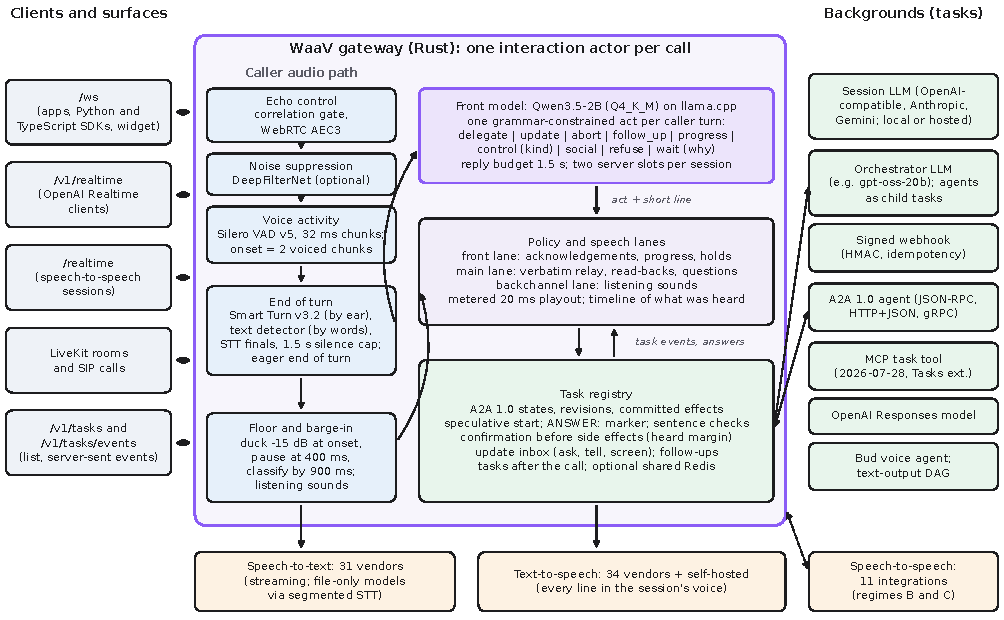
\includegraphics[width=\textwidth]{figures/architecture.pdf}
\caption{Architecture of interaction mode. Clients reach the gateway over several surfaces (left). Each call has
one interaction actor: the caller's audio passes echo control, optional noise suppression, voice activity and
end-of-turn detection, which feed the floor and barge-in machine and, with the transcripts, the front model. The
front model names one act per caller turn; the policy engine schedules speech on three lanes; the task registry
runs requests on background models and agents (right) and relays their answers. Speech-to-text and text-to-speech
(bottom) come from any supported vendor or a self-hosted model; a speech-to-speech provider can replace the
cascade's voice.}
\label{fig:arch}
\end{figure}

\subsection{Overview}\label{sec:sys-overview}

WaaV sits between a client application and speech providers: the client streams audio or text to one endpoint,
and the gateway transcribes it, runs the agent and streams the synthesised reply back, with the providers the
session names~\citep{waav_repo}. Interaction mode is opt-in. A session runs it when the server switch
(\cfg{interaction.enabled}) is on, the session or the operator asks for it, a background exists to run requests,
the speech-to-text provider can end an utterance and keep listening, and a language pack covers the session's
language; otherwise the session receives one \cfg{config_warning} and behaves as without the mode.

Each session has one \emph{interaction actor} that owns the call's state and handles its inbox one message at a
time, running deterministic state machines (duplex engine, floor, policy, lane executor) and spawning every effect
that needs I/O, so timing rules can be tested on a virtual clock~\citep{waav_design}. The design separates three
roles (Figure~\ref{fig:arch}). The \emph{front} decides what each caller turn is and says short lines at once. The
\emph{background} does the requested work as a \emph{task}. The \emph{gateway} owns timing and the words that bind:
it relays the background's answers word for word and words every confirmation, question and failure notice from
templates. The front's prompt forbids it to say a number, date, name or availability the caller did not say, to
predict an outcome, or to say that something is done.

\subsection{Turn-taking, floor and duplex audio}\label{sec:sys-audio}

\paragraph{End of turn.}
Every caller frame is copied, without delaying speech-to-text, into a per-session analyser that runs Silero VAD
v5~\citep{silero_vad} on 32\,ms chunks and confirms the caller's onset after two voiced chunks (64\,ms). A turn ends
when the recogniser ends its segment, earlier when Smart Turn v3.2~\citep{smartturn_repo}, asked 200\,ms into each
pause, is sure the caller has finished, and at the latest after 1.5\,s of silence; release builds also run the
LiveKit text turn detector~\citep{livekit_turndetector} on final transcripts. A thinking pause is \emph{held}: a final
transcript does not end the turn when Smart Turn is unsure (below 0.7) and the words end on one that leaves the
sentence open (``and'', ``to''), and a held turn ends 800\,ms later unless the caller goes on. Turns begun over the
agent and answers to the agent's questions are never held. With \cfg{duplex.eager} the gateway also acts on a likely
end of turn before the final transcript by starting a provisional background run (Section~\ref{sec:sys-tasks}).

\paragraph{Floor and heard audio.}
The gateway reports who holds the floor (\texttt{user}, \texttt{assistant}, \texttt{both} or \texttt{none}). The
agent's audio leaves through a metered pump that paces 20\,ms frames on a playout clock and holds everything beyond
a short lead (150\,ms on a WebSocket, 40\,ms in a LiveKit room), so a duck or a cut acts on audio not yet heard.
From delivered frames and the client's playback reports the gateway keeps a timeline of what the caller heard; it
decides when a spoken ``yes'' binds (Section~\ref{sec:sys-hitl}), what ``say that again'' repeats, and what the
background is told: a line the caller cut off enters the history only up to its last heard word.

\paragraph{Barge-in and listening sounds.}
At the caller's onset over the agent the analyser \emph{ducks} the agent's voice ($-15$\,dB over 60\,ms), a reaction
to sound, not words. An overlap of 400\,ms pauses the agent, and by 900\,ms after the onset the overlap is classified
as an interruption, a backchannel or background speech; a caller still speaking then takes the floor. Meanwhile the
front reads the recogniser's interim results (Section~\ref{sec:sys-front}), so ``stop talking'' can cut the agent
before the turn ends. A cut affects only the utterance that is playing: queued lines return to the policy engine and
tasks keep running. During long turns the agent makes listening sounds (``mhm'', ``I see'') from the language pack,
rendered at session start in the session's voice, played 3\,dB below speech on their own lane and kept out of the
history; one plays at a pause only when Smart Turn says the caller has not finished, after enough of the caller's
speech and not too soon after the last one, and never while private details are given or, by default, on phone lines.

\paragraph{Echo.}
A transcript filter drops transcripts that repeat what the agent just said; a correlation gate finds the delivered
audio returning in the caller's channel (up to 1\,s later) and does not count it as an onset; and WebRTC's AEC3
canceller~\citep{webrtc_src} turns on automatically for phone lines, clients without echo cancellation and after
repeated echo. DeepFilterNet noise suppression~\citep{schroeter2022deepfilternet} is optional.

\subsection{The front model}\label{sec:sys-front}

\paragraph{Model and prompt.}
The front model is Qwen3.5-2B~\citep{qwen35_2b} (Apache-2.0), without thinking and quantised to 4 bits, served by
llama.cpp's \texttt{llama-server}~\citep{llamacpp}, which the gateway can start, supervise and restart. It was chosen
after a bake-off of small open models on labelled decisions~\citep{waav_design}; an earlier plan for a rule router as
the front was dropped, and there is no rule-based fallback. The prompt has a stable prefix (persona, act definitions,
policies, hard rules) that the server caches across calls, a per-call header (the caller's name and preferences, and up
to three remembered facts), and a per-decision observation: what the caller heard of the agent's last line, the
caller's words with marks such as \emph{interrupting you}, one line per relevant task, and the acts allowed now. Text
from the call is quoted as data.

\paragraph{Acts.}
The model answers with one JSON object. The reply is prefilled with \verb|{"act":"| and a grammar built for each decision
admits only the acts legal at that moment; because no two act names share a first letter, the first generated character
names the act and the gateway can act before the line is complete. Table~\ref{tab:acts} lists the acts. The short line
that goes with \texttt{delegate} is constrained to the persona's openers and inquiry phrases plus spans of the caller's own
words (``Okay, let me check whether your bag is included in the fare''): it can restate the request but not assert an
outcome. A decision has \cfg{front.total_budget_ms} (1.5\,s) for its whole reply; a late decision is not guessed, and the
caller is asked to repeat. Every decision is logged with the observation the model was shown.

\begin{table}[t]
\centering
\caption{The front model's acts. Which acts are allowed depends on the state of the call.}
\label{tab:acts}
\footnotesize
\begin{tabularx}{\textwidth}{@{}>{\raggedright\arraybackslash}p{1.9cm}>{\raggedright\arraybackslash}X>{\raggedright\arraybackslash}p{5.6cm}@{}}
\toprule
Act & When the front chooses it & What the gateway does \\
\midrule
\texttt{delegate} & the caller wants something the background must find out or do & starts or adopts a task; says the acknowledgement \\
\texttt{update} & the caller changes or adds to running task $t_N$ (``no, Thursday'') & revises the task; restates only the new value \\
\texttt{abort} & the caller wants $t_N$ stopped & cancels it and words the true outcome \\
\texttt{follow\_up} & the caller asks about, or wants more of, finished $t_N$ & answers from the stored result or continues $t_N$ on its agent \\
\texttt{progress} & the caller asks how $t_N$ is going, or how to hear about it & says the status; may set how $t_N$ is announced \\
\texttt{control} & the caller steers the call itself (stop, hold, repeat, slower, \ldots) & applies the control (Section~\ref{sec:sys-controls}) \\
\texttt{social}, \texttt{refuse} & greeting, thanks, small talk in scope; out of scope or unsafe & says the persona's matching line \\
\texttt{wait} & mid-thought, a continuer (``uh-huh''), side talk, or nothing new & says nothing \\
\bottomrule
\end{tabularx}
\end{table}

\paragraph{Readings, slots and interims.}
When the caller's words may answer something the agent asked, the gateway sends a short \emph{reading} request with the
question and the possible labels (for a confirmation: \texttt{yes}, a weak \texttt{okay}, \texttt{no}, \texttt{change},
\texttt{cancel}, \texttt{other}); readings also decide whether a request repeats a recent task and which language the
caller spoke. No phrase list decides what the caller meant. Each session holds two server slots: one for decisions on the
caller's turns, one for words said over the agent, readings and narrations. At the start of each agent line the second
slot is primed with the over-speech prompt minus the caller's words (\emph{client-rendered interims}), so an interim
transcript sends only its words; it cuts the agent only on a sure reading (a \texttt{stop} at once, a \texttt{hold} when
the next interim agrees).

\paragraph{The narrator.}
The front also words task updates: one sentence of at most 20 words from the last two lines of the call, a task's title
and its result. It is spoken only if every number and name in it appears in the result, the title or the caller's last
words; otherwise the update waits for its next slot. There is no template fallback.

\subsection{Policy and speech}\label{sec:sys-policy}

The policy engine is a pure state machine, \texttt{step(now, input)} $\to$ actions, that decides who speaks, what and when,
on a \emph{front} lane (acknowledgements, progress, holding lines), a \emph{main} lane (relayed answers, read-backs,
questions) and a \emph{backchannel} lane~\citep{waav_design}. After a delegated turn the acknowledgement is due 300\,ms
after the end of the turn; when the background's first answer sentence has recently arrived within 700\,ms (median of at
least three turns), the gateway waits until 700\,ms and skips the acknowledgement if the answer is ready. By 2\,s the caller
hears something. The background's answer is spoken in its own words, sentence by sentence as it is written, and never passes
through the front: a prompted background begins its final answer with a line \texttt{ANSWER:}, text before it and rounds
that end in a tool call are never spoken, and each sentence is dropped if it contains a link, a number of seven or more
digits the caller did not give, a prompt label, or a restatement of the background's instructions. While a task runs and
nobody speaks, the agent says progress lines on real changes, a holding line after 8\,s of silence, and later offers to keep
waiting or stop.

\subsection{Tasks}\label{sec:sys-tasks}

\paragraph{Task model.}
A task is one piece of work the caller asked for, with a lifetime of its own: it survives barge-in, corrections, a dropped
connection and, if it may have side effects, the end of the call. It has a short alias (\texttt{t1}) the front refers to, a
\emph{revision} that rises with each correction, a kind (\texttt{lookup} or \texttt{action}), a state following
A2A~\citep{a2a_spec} (\texttt{submitted}, \texttt{working}, \texttt{input\_required}, then \texttt{completed},
\texttt{failed}, \texttt{cancelled}, \texttt{rejected} or \texttt{unknown}), and its \emph{effects}: none committed, a list
of what was done, or unknown. Stopping a run never undoes an effect, so cancellations and failures always report them.
Clients receive \texttt{task\_created}, \texttt{task\_progress}, \texttt{task\_question}, \texttt{task\_output},
\texttt{task\_result} and \texttt{task\_cancelled} events.

\paragraph{Speculative start.}
When the policy asks the front for a decision with \texttt{delegate} allowed, the background run starts in the same step on
the caller's words, or earlier at an eager end of turn. Nothing from this provisional run is spoken or sent, and
side-effecting calls wait, until the act settles: \texttt{delegate} adopts the run as the task, any other act discards it.
Speculation is off for backgrounds that run their own tools and for the OpenAI Responses API, where a dropped run is billed.

\paragraph{Corrections and cancellation.}
An \texttt{update} revises the running task; before a side-effecting tool runs, a gate refuses a call made under a stale
revision, and a remote run is restarted on the corrected request. A request that nearly repeats a running or just-committed
action is held with ``Do you want me to change it, or is this a second one?''. A cancellation of a task that may have side
effects counts only when the backend confirms it; otherwise the caller hears ``I've stopped it, but I can't confirm whether it
had already gone through.'' Tools are HTTP endpoints called with an HMAC signature and, for side effects, an idempotency key
derived from the task and its revision; a timeout on such a call is an unconfirmed effect and is not retried.

\paragraph{After the call.}
A task that may change something, or whose result someone can read, runs on after a hang-up: a caller whose connection
dropped may return within 60\,s to hear the outcome, and otherwise it is pushed, signed, to the operator's endpoint.
With a shared Redis several gateway processes share tasks under leases. \texttt{GET /v1/tasks} and its server-sent event
stream let a dashboard follow the work independently of the voice channel.

\subsection{Backgrounds and the open task protocol}\label{sec:sys-backgrounds}

A task runs on the session's own language model (any OpenAI-compatible server such as \texttt{llama-server} or vLLM, or
OpenAI, Anthropic or Gemini), on a Bud voice agent, on a processing graph that ends in text, or on a remote backend that the
operator declares in the server configuration, where its address and secret stay: a \textbf{signed webhook} that receives
\texttt{task}, \texttt{answer} and \texttt{cancel} messages and replies with progress, effect, question, result and control
events; an \textbf{A2A 1.0 agent}~\citep{a2a_spec} over JSON-RPC, HTTP+JSON or gRPC, with streaming and push notifications,
whose \texttt{input-required} state becomes a question to the caller and \texttt{auth-required} a sign-in link on screen; an
\textbf{MCP task tool}~\citep{mcp_spec} on the 2026-07-28 revision with the Tasks extension, whose elicitations become
questions and progress notifications progress lines; or an \textbf{OpenAI Responses} model in background mode. Each entry has
a concurrency limit, a timeout and a circuit breaker with an optional fallback.

\paragraph{Orchestrator and child tasks.}
With \cfg{tasks.orchestrator} the requests go to a larger model, for example gpt-oss-20b~\citep{openai2025gptoss}, whose tools
are the session's agents, described by their A2A Agent Cards and MCP tool lists. Calling an agent starts a \emph{child task}
and returns at once, so several agents can work in parallel; a finished child's result returns to the orchestrator as a task
update. Every task event carries \texttt{parent\_id}, \texttt{agent} and a \texttt{trace\_id}, which also travels to agents
and tools in a W3C \texttt{traceparent} header~\citep{w3c_tracecontext}. Agent calls that may change something pass the same
confirmation gate as tools.

\paragraph{Updates and follow-ups.}
A finished task's full result is \emph{published} at once as \texttt{task\_output}, with structured data and artifacts, but
\emph{spoken} only at a slot: nothing of the agent's is playing, the latest request has its answer, no question is open and the
caller is silent. After 4\,s of quiet the update is said; right after an answer, \cfg{tasks.announce} decides between offering
it (``I've got the answer on your request to book the flight. Want it now?''), saying it, or leaving it to the screen, and the
caller can choose per task. An agent's question whose deadline cannot wait breaks in at the next clause boundary (``Quick
question.'') and the interrupted answer resumes afterwards. A finished agent task stays addressable for 30 minutes with its
continuation handle, so ``when does it land?'' is answered from the stored result or continued on the same agent.

\subsection{Confirmations and human in the loop}\label{sec:sys-hitl}

A tool declared with side effects is held before its request is sent. The gateway reads the call back from its exact arguments,
in the tool's confirmation phrase or its author's template (``To confirm: book a table for 4 at Rosa's. Do you want me to do
that?''), and the caller answers by voice or on screen. A spoken ``yes'' counts only if it began at least 150\,ms after the
read-back was heard in full; for an irreversible tool a weak ``okay'' is asked again; one question is open at a time, the same
call under one revision is asked once, and a decline or timeout means the request is never sent. The background can ask for a
choice or value through a built-in \texttt{ask\_caller} tool under the same rule. Forms, sign-in links and sensitive values (card
numbers, PINs, passwords, one-time codes) never go over the voice channel: they are put on the client's screen, and while such a
value is asked the speech-to-text provider receives silence of the same length, so a value said anyway reaches neither a
transcript nor a vendor. On a phone line the caller can confirm on the keypad (1 or 2) and type sensitive values. A session
without a screen declines such questions with an explicit line.

\subsection{Conversation controls}\label{sec:sys-controls}

Requests to steer the conversation become one \emph{control} from a closed list: \texttt{stop}, \texttt{hold} (stop
speaking, keep tasks running), \texttt{resume} (from the first sentence not heard in full), \texttt{repeat} (the last line
heard, or only its number or code, optionally slower or louder), \texttt{not\_heard}, \texttt{spell}, \texttt{clarify},
\texttt{rate} and \texttt{volume} (one step within the operator's bounds), \texttt{verbosity}, \texttt{language} (to a language
the operator lists, with a reviewed pack), \texttt{voice}, \texttt{backchannels}, \texttt{updates}, \texttt{to\_screen},
\texttt{end} and \texttt{human} (a transfer to a person over SIP or a signed webhook). Whoever asks (the caller, through the
front's \texttt{control} act; the client application; the orchestrator, whose request is applied only when it quotes words of
the operator's prompt or the caller; or a remote agent), one executor applies the control and answers
\texttt{control\_applied} as applied, partial, unsupported or refused. A control that cannot be applied in full is said so
(``Sorry, I can't change my speed on this line.''), and each control updates a versioned conversation state that every
background receives.

\subsection{Failures}\label{sec:sys-failure}

A health watcher, fed by the code paths that report failures and never by the caller's words, marks the recogniser, the front,
the background or the voice as degraded, for example when the background shows no sign of life within 2.5\,s while the caller
waits. The agent then says so in short lines rendered at session start in its own voice (``Sorry, my systems are acting up. Bear
with me a moment.''), at most three per outage, says when it is back, and if the outage lasts 30\,s after the first line says
goodbye and closes the session with \texttt{session\_failed} and the list of live tasks. The lines never name a vendor.

\subsection{Providers and surfaces}\label{sec:sys-surfaces}

WaaV puts 44 speech vendors behind one API (31 speech-to-text, 34 text-to-speech plus self-hosted synthesis, 11
speech-to-speech integrations)~\citep{waav_repo}. Interaction mode runs on \texttt{/ws} sessions (typed in the Python and
TypeScript SDKs), on Bud voice agents over the OpenAI Realtime protocol, in LiveKit rooms and on SIP calls, which are
treated as phone lines (echo cancellation and keypad answers on, listening sounds off). On \texttt{/realtime} a
speech-to-speech provider can keep its own voice and turn-taking while WaaV is its background: the provider gets one
function, \texttt{waav\_delegate}, for anything to look up or do. Either the gateway has the provider say confirmations and
results in checked words (OpenAI, Grok, Deepgram Voice Agent and others) or the provider stays the front and the gateway
speaks only what committed something (Gemini Live, Nova 2 Sonic). Because the gateway can monitor but not prevent what such
a provider says, the operator must accept each provider explicitly; a completion claim no task supports or a number nobody
gave raises \texttt{unverified\_claim} and optionally a spoken correction. Personas, language packs added as data (English is
built in) and an optional caller memory (at most ten short facts, never numbers or codes) complete the operator's surface.
